\chapter{Circuit Design}
\label{chapter:circ_design}

The symbol and interface signals of the sample rate converter design is
presented in Fig.~\ref{fig:bd_top_iface}. The data input and output signals are
$x$ and $y$, respectively, and the sample rate clocks are $x\_clk$ and $y\_clk$,
respectively. The definition of all interface signals is presented in
Table~\ref{tab:top_iface}.

\begin{figure}[!htb]
  \centering
  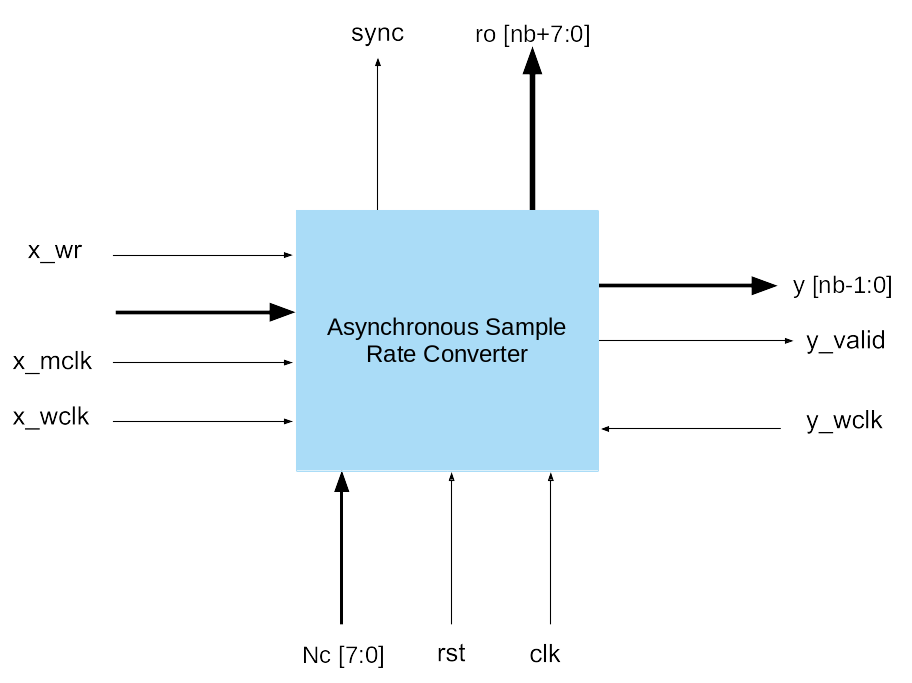
\includegraphics[width=0.7\textwidth]{Figures/asrc_iface_bd.png}
  \caption{Asynchronous sample rate converter interfaces block diagram.}
  \label{fig:bd_top_iface}
\end{figure}

\begin{table}[!htbp]
  \centering
  \caption{List of asynchronous sample rate converter interface signals.}
  \label{tab:top_iface}
  \begin{tabular}{|c|c|p{0.7\linewidth}|}
    \hline 
	{\bf Name} & {\bf Direction} & {\bf Description} \\ \hline
        \hline
	clk & Input & System clock input.\\ \hline
	rst & Input & Active high synchronous reset.\\ \hline
        \hline
        Nc [7:0] & Input & Number of input audio channels.\\ \hline
        \hline
        x [nb-1:0] & Input & Input sample.\\ \hline
        x\_wclk & Input & Input word clock, with frequency equal to the input sample rate.\\ \hline
        x\_mclk & Input & Input master clock. Should be $2^N$ times faster than x\_wclk, where N is an integer
        greater than Nc.\\ \hline
        x\_wr & Input & Input sample write enable.\\ \hline
        \hline
        y [nb-1:0] & Output & Output sample.\\ \hline
        y\_wclk & Input & Output word clock, with frequency equal to the output sample rate.\\ \hline
        y\_valid & Output & Output sample valid. Should be used as an enable to an output
        sample register.\\ \hline
        \hline
        ro [nb+7:0] & Output & Sample rate convertion ratio signal. Represented in format
        8Qnb.\\ \hline
        sync & Output & Active high when the converter has stabilized.\\ \hline
  \end{tabular}
\end{table}

The ASRC is divided in three modules: the Input Data Memory, the Ratio Estimator
and the Resampler. Additionally, a simple positive edge detector circuit is
needed to start the execution of some modules. A block diagram of the
ASRC with its three modules is presented in Fig.~\ref{fig:bd_top}.

The core works in three different clock domains and all figures present the
signals in three different colors, with green arrows indicating signals in
$x\_mclk$'s domain, blue arrows for signals in $y\_wclk$'s domain, and black
arrows for signals in $clk$'s domain. This is important as wherever there is a
clock domain crossing there needs to be a suitable synchronizer circuit.

\begin{figure}[!htb]
  \centering
  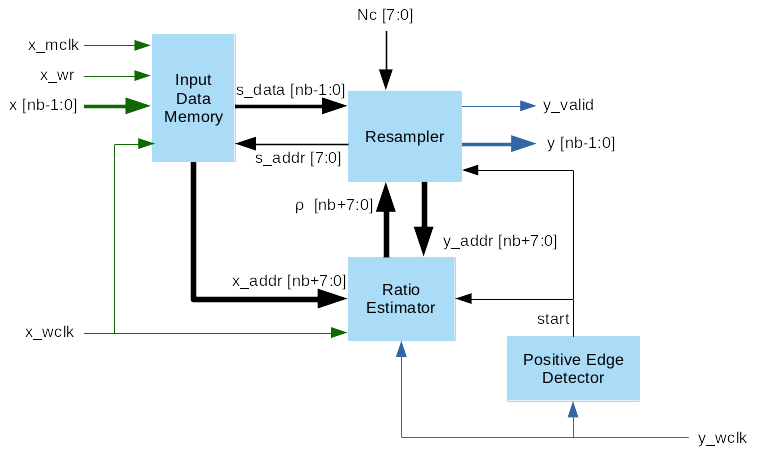
\includegraphics[width=0.8\textwidth]{Figures/asrc_top_bd.png}
  \caption{Asynchronous sample rate converter top block diagram.}
  \label{fig:bd_top}
\end{figure}

\section{Data Memory}
\label{section:data_mem}

To store the input samples, a data memory is used. This data memory should be a
dual port Random Acess Memory (RAM) capable of working at two different clock
domains. The block diagram of this memory and the auxiliary components to access
is presented in Fig.~\ref{fig:bd_datamem}.

\begin{figure}[!htb]
  \centering
  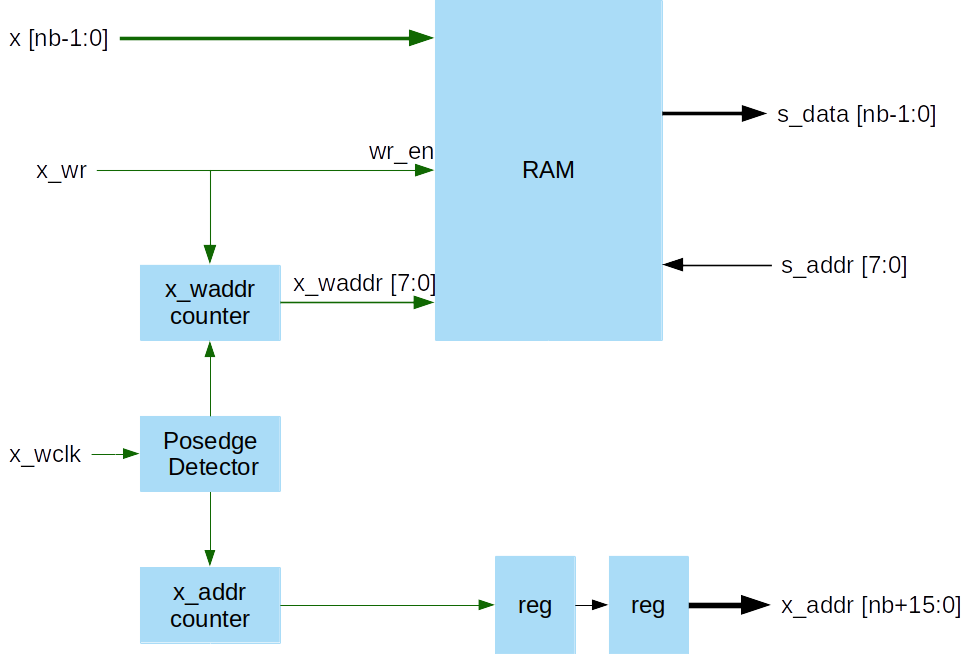
\includegraphics[width=0.8\textwidth]{Figures/asrc_datamem_bd.png}
  \caption{Data memory module block diagram.}
  \label{fig:bd_datamem}
\end{figure}

In the input clock domain, the samples $x$ are stored in the position given by
$x\_waddr$ at the rate of $x\_mclk$. The write address counter $x\_waddr$ is
incremented at $x\_mclk$'s rate, whenever $x\_wr$ is active.
In the time domain of the system clock, the
samples are read by accessing the position given by $s\_addr$. For each output
clock pulse, the input samples needed to perform the filtering are read from the
memory at the system clock rate. For a multiple channel input, to obtain the
next sample of a certain channel, the address $s\_addr[n+1]$ is given by
\begin{equation}
  s\_addr[n+1] = s\_addr+Nc.
  \label{eq:datamem_nextsample}
\end{equation}

Since the accumulators do not stop or reset during the execution of the
conversion, they wrap around creating a circular memory. When there is a stream
of input samples, the newer ones will overwrite the older ones which will not be
used anymore in the time-finite fractional delay filter.  On average the write
and read pointers increment at the same rate, which is guaranteed by the Ratio
Estimator block.

This module also contains an additional counter, $x\_addr$. This counter
is similar to the $x\_waddr$ counter, with the difference that it is
not controlled by $x\_wr$. This counter is used by the ratio estimator
described in Section~\ref{section:ratio_est}, as an parameter used
to adjust the sample rate conversion ratio.


\section{Ratio Estimator}
\label{section:ratio_est}

Since the sample rate converter is asynchronous, the frequency of the input and
output clocks can change over time. Furthermore, their frequencies can also take
any value in the supported range. The frequencies of the data clocks are unknown
by the core but their ratio must be computed. The Ratio Estimator is the module
that computes the ratio between the periods of the data clocks, and its block
diagram is shown in Fig.~\ref{fig:bd_ratioest}.

\begin{figure}[!htb]
  \centering
  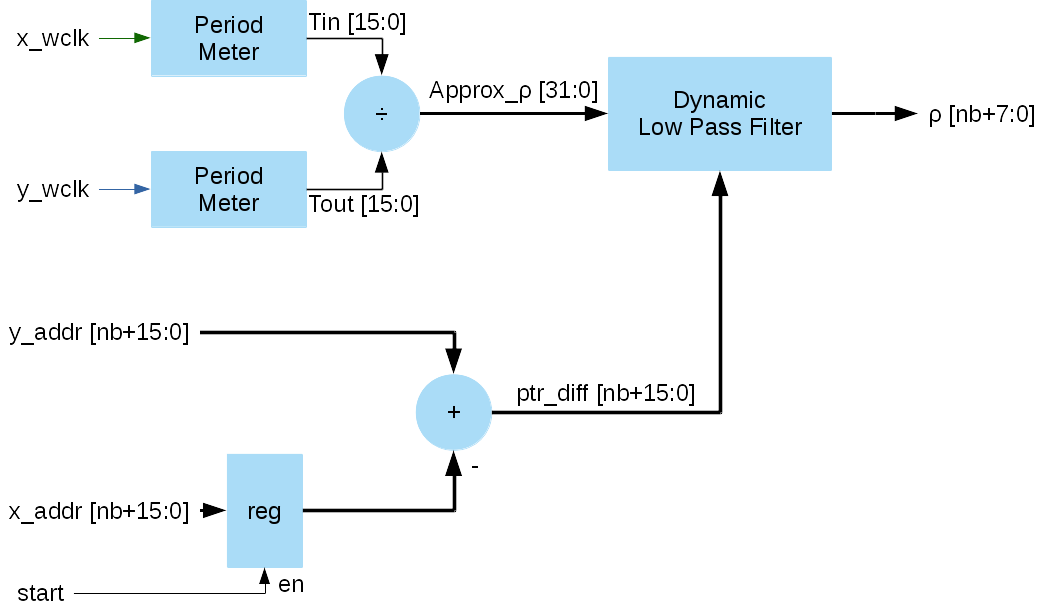
\includegraphics[width=0.8\textwidth]{Figures/asrc_ratioest_bd.png}
  \caption{Ratio Estimator module block diagram.}
  \label{fig:bd_ratioest}
\end{figure}


The Period Meter block uses a counter to obtain a relative value $T_{count}$ of
the period of the data clocks. Since the counter is incremented at the system
clock rate $f_{sys\_clk}$, an approximate value of the data clock period $T_d$
is given by

\begin{equation}
  T_d = \frac{T_{count}}{f_{sys\_clk}}.
  \label{eq:samp_rate_period}
\end{equation}

The ratio $\rho$ between the input and output clock frequencies $f_{in}$ and $f_{out}$
is defined by

\begin{equation}
  \rho = \frac{f_{out}}{f_{in}}.
  \label{eq:rho_teo}
\end{equation}

Combining Equation~(\ref{eq:samp_rate_period}) and~(\ref{eq:rho_teo}), an
approximate value of $\rho$ can be computed by

\begin{equation}
  \rho  = \frac{T_{count\_in}}{T_{count\_out}}.
  \label{eq:rho_hw}
\end{equation}

The value of $\rho$ can be computed in hardware without knowing any clock
frequencies. However, since the counter is only able to count integer values,
the periods of the input and output clocks are imprecise.  For the same clock
frequency the value $T_{count}$ can vary each time it is determined, with an
absolute error of 1 unit. It should be noted that the resolution of the counter
increases with the frequency of the system clock: a higher system clock
frequency leads to a lower error in $T_d$.

These errors lead to an imprecise value of $\rho$, leading not only to an error
in the conversion done in the resampler module, but also to having the read and
write pointers in the data memory module incrementing at different average
speeds, which eventually may cause the buffer to underflow or overflow. The
dynamic low pass filter is the block which solves this problem, as it stabilizes
the deviations of the approximate result of $\rho$, obtained according to
Equation~(\ref{eq:rho_hw}), obtaining the mean value instead. The structure of
the dynamic low pass filter is not given at this stage. It will simply be stated
that when there is a high deviation of the approximate $\rho$, the filter's
cuttoff frequency rises, as it assumes there was a change of the input and/or
output clock frequencies. When the deviation lowers, the filter's cuttoff
frequency lowers as well, being less sensitive to the small deviations of the
approximate $\rho$ caused by quantization and period counting errors. A
correction parameter that takes into account the difference between the read and
write pointers of the input data memory adjusts the value of $\rho$. The read
pointer increment rate is changed to keep the difference between the pointers
constant, for example, ensuring that the read and write pointers have a distance
equal to half of the memory's size.


\section{Resampler}
\label{section:resampler}

The resampler is the main module of the sample rate converter and executes the
conversion algorithm. This complex module is split into three submodules: the
\textit{address generator}, the \textit{coefficient memory} and the
\textit{multiply-accumulate} submodule, which are explained in the next
subsections. A block diagram of the resampler is presented in
Fig.~\ref{fig:bd_resampler}.

\begin{figure}[!htb]
  \centering
  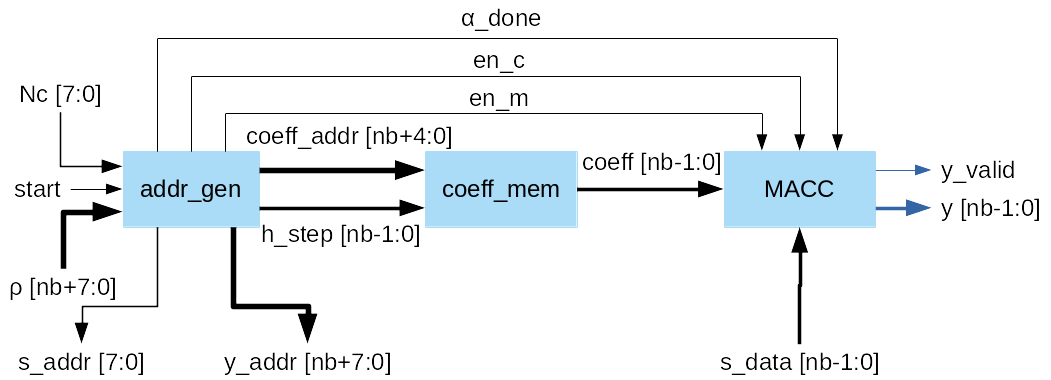
\includegraphics[width=0.8\textwidth]{Figures/asrc_resampler_bd.png}
  \caption{Resampler module block diagram.}
  \label{fig:bd_resampler}
\end{figure}

\subsection{Address Generator}
\label{subsection:addr_gen}

The address generator is the submodule responsible for computing the addresses
of the input samples needed to compute the output sample. As explained in
Sections~\ref{section:fd_filter} and~\ref{section:output_computation}, there
are two main steps needed to compute an output sample: (1) center the filter at
the time of output sample to be computed; (2) compute the input samples and
correspondent filter coefficients and perform the filter convolution operation.

To center the filter at the time of the output sample to be computed, an alpha
computation submodule is used. This submodule computes the time of the current
output sample to be computed in the form of a fractional address $y\_addr$,
which is incremented by a factor $1/\rho$ at the output sample rate.

Additionally, there is the need to know the distance in time (normalized to the
input's sample rate) between the current output sample and the closest input
sample, as this distance defines the first coefficient to be used for each side
of the symmetric filter. This distance is called $\alpha$ and is computed by
assuming that there is an input sample $x[n]$ for all integer values of $n$, and
that $1-\alpha$ is the fractional distance between the output sample and the
closest input sample.

Finally, to adapt the filter's shape, ensuring that it has a cutoff frequency
defined by Equation~(\ref{eq:filter_cutoff}), a parameter $h\_step$ is defined
by normalizing the cutoff frequecy to the input sample clock frequency:

\begin{equation}
  h\_step = min(1, \rho).
  \label{eq:h_step}
\end{equation}

With the value of $h\_step$ and $\alpha$, as well as the integer part of
$y\_addr$, it is possible to determine all of the needed addresses for the input
samples and correspondent coefficients.

To get the input samples' addresses a simple counter submodule
(\textit{s\_addr  computation}) is used.
The integer part of $y\_addr$ is used as the base of the address computation.
Knowing that consecutive input samples of the same channel have the distance defined by
Equation~(\ref{eq:datamem_nextsample}), it suffices to accumulate this distance
from the offset of the current channel to get all needed input sample addresses
that come after (or to the right of) the output sample instant. When the right
side is completed, the left side is computed by negative accumulations from the
channel offset, getting the addresses of all input samples before the output
sample instant. When both sides are done, the channel offset is incremented and
the process is repeated for the next channel. This means that one channel is
computed at a time, allowing the use of a single multiply-accumulate unit to
compute the output samples for all channels.


To get the coefficients' addresses, another accumulator is used. The value of
$\alpha$ is used as the initial value in order to align the input sample to its
filter coefficient. Since an increment of one input sample corresponds to a
increment of $h\_step$ in the coefficient function, $h\_step$ is used as the
accumulation value. These accumulations will be done until the filter is no
longer defined, which happens when the accumulator reaches or overcomes the
final address of the coefficients memory. After these accumulations are done,
there is a side switch, and the accumulations restart, with the complement
$1-\alpha$ as the initial value and the same increment of $h\_step$. This module
also produces two flags, $en\_m$ and $en\_c$, to enable accumulations and reset
the accumulator when the channel is done, respectively.

\subsection{Coefficient Memory}
\label{subsection:coeff_mem}

To get the filter's coefficients, the simplest way is to have a lookup table
with them already pre-computed using a Read Only Memory (ROM).  Because
of the high precision needed the ROM would be too large.  To solve this problem,
a simple linear interpolator is used. Assuming that a certain coefficient
$h[i+\Delta]$ is needed, $h[i]$ and $h[i+1]$ exist in the lookup table, and
$\Delta$ is a fractional positive distance to $i$, the coefficient is obtained
by

\begin{equation}
  h[i+\Delta] = h[i] + \Delta (h[i+1]-h[i]).
  \label{eq:coeff_interpol}
\end{equation}

\subsection{Multiply-Accumulator}
\label{subsection:macc}

This submodule is a simple accumulator, done with a register and an adder. Its
input is the product between the coefficient and the input sample as defined by
Equation~(\ref{eq:macc}). Its initial value is set by directly loading (not
accumulating) the first product.

The final register, which produces the output $y$, is enabled only when all
accumulations have finished. This ensures that $y$ never has an intermediate
value. This output is updated at the output sample rate but lives in the system
clock domain. Therefore a synchronizer is further needed to convert it to the
$y\_wclk$ clock domain.
